\documentclass[12pt,letterpaper,onecolumn]{article}
\usepackage{graphicx}
\usepackage{minted}
%\usemintedstyle{arduino}
\setminted[c]{linenos, frame=lines,style = arduino}
\setminted[cpp]{linenos, frame=lines, style = xcode}
\usepackage{mathptmx}
\newcommand{\titlefont}{\fontfamily{ptm}\fontseries{b}\fontsize{16pt}{\baselineskip}\selectfont}
\newcommand{\authorfont}{\fontfamily{ptm}\fontseries{b}\fontsize{14pt}{\baselineskip}\selectfont}
\newcommand{\zwfont}{\fontfamily{ptm}\fontsize{12pt}{\baselineskip}\selectfont}
\newcommand{\codefont}{\fontfamily{phv}\fontsize{11pt}{\baselineskip}\selectfont}
\newcommand{\headfont}{\fontfamily{ptm}\fontseries{b}\fontsize{12pt}{\baselineskip}\selectfont}
\usepackage{geometry}
\geometry{left = 1.0in,right = 1.0in,top = 1.0in,bottom = 1.0in}
\title{\titlefont Report for Lab 3\vspace{300pt}}
\author{\authorfont Muhan Li\\ \authorfont Man Sun\\ \authorfont Mingxiao An}
\date{}
\usepackage{titlesec}
\titleformat*{\section}{\headfont}
\titleformat*{\subsection}{\headfont}
\usepackage{xcolor}


\begin{document}
	\maketitle
	\thispagestyle{empty}
	\vspace{40pt}
	\hfill \newline
	\textbf{Statement}: we promise that all of the work in this lab and report are finished by ourselves.\\
	\textbf{Sign}: Muhan Li, Man Sun, Mingxiao An.\\
	\newpage
	\tableofcontents
	\newpage
	\section{ABSTRACT}	
	%	The abstract should provide a brief overview of the report - one paragraph at most. 
	%	
	%	It should provide a summary of the main specific points for the introduction, the main tests and experiments, the results, and the conclusions. It is called an abstract because you can literally "abstract" sentences from the other sections. 
	%	
	%	Once again, this is not a narrative of your experiences as you executed the design.  The abstract should mirror (albeit in a very condensed way) the content of your report.	
		In this report, we will give a brief introduction on the purpose and tools used in the lab, a very
detailed discussion of the lab. the testplan we will apply, the result of the lab as well as its analysis,
the errors we met when doing this lab and the analysis, and the summary and conclusions of the
whole lab and report. We will include a little user manual in the detailed discussion. We will also hard copy our code used in this lab to the Appendices.
	\section{INTRODUCTION}
	%	Brief introduction and overview of the purpose of the lab and of the methods and tools used - one to two paragraphs at most.
		This lab is the last lab. The specification will all be designed by ourselves. This lab aims to improve our understand of formal design process. We will also need to show our imagination and creativity in design with Arduino in this lab.
\newline
We designed a shell game, and implemented it to the arduino platform with various elements, including two arduino UNO board, two XBee shields, a joystick shield, a lcd1602, a buzzer, and a tilt switch.
	\section{DISCUSSION OF THE LAB}
	%	This section should include the following:
	%	
	%	Brief Design Specification - In this subsection you will textually describe your client's requirements.  What does he or she need in the project you are developing.  If you are incorporating extra features or capabilities, please describe them clearly in this section.
	%	
	%	Overall summary description of the module - 2-3 paragraphs maximum
	%	
	%	Specification of the public interface to the module
	%	
	%	Inputs
	%	Outputs
	%	Side effects - what outside variables did the module change
	%	
	%	Pseudo English description of algorithms, functions, or procedures
	%	Error handling
	%	
	%	Hardware Implementation
	%	
	%	Draw the schematic / logic diagram of how you connected the parts...switches, chips, LEDs etc.
	%	
	%	Use standard symbols for simple electronic parts and appropriately labeled boxes for larger parts. Should be a cleaned-up "picture" of what your breadboard and components actually look like
	%	
	%	Do not actually take a picture and submit this.
	%	
	%	Software Implementation
	%	
	%	What is your design????
	%	
	%	Present your design starting from a top level functional view and potentially block diagram or high level architecture. 
	%	
	%	Refine that view to present and explain each of the modules that comprise the major functional blocks. 
	%	
	%	Discuss the flow of control through the design. 
	%	
	%	Identify and discuss the specific modules you have implemented in your design. Explain your design choices.  
		\subsection{Brief Design Specification}
\subsubsection{Overall summary description of the module}
This module is a box-guessing game designed by ourselves. The input is received from a joystick, four direction buttons and one tilt button. The user can control and choose boxes with joystick and direction buttons. The user can also turn the screen off by flipping the tilt button. The game screen is a LCD screen connected to one of the two Arduino boards. The user's command and movement will be transfered from one board to another and will be reflected on the serial monitors.

\subsubsection{Specification of the public interface to the module}
\paragraph{Inputs, Outputs and Side Effects}
\hfill \newline
Since there are two boards in our module, we will introduce the two boards separately.
\subparagraph{Master}
\hfill \newline
The input of the master board is a joystick(containing four directions), and four direction buttons. These inputs are received by passing pointers to functions that realize the reactions to different buttons and directions of joystick movement to the public interface of the joysticks and buttons.Users can use joystick to move the cursor to select the box they want to guess before the game starts and the correct box they think in the open box phase. They can also use the joystick to modify the settings. To enter the setting page, they will need to push the up button before the game starts. They can push the right button to confirm after they choose the box to guess, before and after they select the box as their guess, after they finish setting, and after they finish reading the tutorial. They can push the down button before the game starts to read the tutorial and to exit the tutorial page. \\
\hfill \newline
Their commands will be transfered to the slave board through serial port, so the output of the master board would be serial that can be checked on the serial monitor on PC. It will send a code number for each commands followed by nothing or some digits or string to be delivered. \\
\hfill \newline
Each time the user moves the joystick or pushes a button, some parameters will be changed to help to compute the new display of the screen.
\subparagraph{Slave}
\hfill \newline
The input of the slave board is from the serial port. At the beginning of each time of transmission, a digit code for the type of command will be sent. According to the type of the command, different number of digits or string will be sent. A tilt button also serves as one part of the slave board's input.\\
\hfill \newline
The output of the slave board is its LCD screen and a buzzer. Also, it will print what it will do on the serial monitor after each movement.\\
\hfill \newline
Depending on the command it receives from the serial port and the tilt button, it will change different local variables such as the number of boxes, the speed of swapping, the cursor position, etc.

\paragraph{Pseudo English description of algorithms, functions, or procedures}
\hfill \newline
We use multi-file to build the module, and each files are perfectly separated from others. Each can be seen as a independent utility, so we will introduce the functions in terms of files.

\subparagraph{Command}
\hfill \newline
We made the two boards communicate through the wireless network supported by XBee, but in software realization, we used a self-defined code. We use enumeration to make the code more clearly. Then we define a function to receive these command code, and switch the received code to corresponding command reactions.

\subparagraph{Display}
\hfill \newline
We realize all the refreshing functions in this file. We mainly realize these functions by using public interface provided by LCD in Arduino.

\subparagraph{Constant}
\hfill \newline
We define all the constants that won't be changed by the game players in this file. Other files will include this file to use these constants.

\subparagraph{Game}
\hfill \newline
For the fact that we set the game to loop forever -- until the boards are plugged off. We define the procedure of a round of game in this file. The specific procedure in top level can be found in our flowchart(figure[\ref{fig:flow}]). We transmit commands by calling functions from the command file and delay for a period of time. The delay time for most of the command are fixed. For switching(moveSwap() in code) command, we need to modify the delay time according to the speed. That is because we need to send this command repeatedly for many times. If we send them too frequently, the buffer for the slaver board will be overflow because the command will only be read after the previous one is finished. But if we send it too slowly, the movement of the boxes will seem sluggish.

\subparagraph{Graph}
\hfill \newline
In order to display such self-defined characters as boxes, cursor, arrows, we will need to use the public interface LiquidCrystal::createChar(). To use this interface, we will need to pass a pointer to an array of byte, a type defined by Arduino. The array is consisted of binary numbers, where each bit represents a pixel in the $ 8\times 5 $ character symbol (0 for blank and 1 for black). In this file, we defined all the arrays we need in this game. In display file, we only need to include this file to create new characters.

\subparagraph{Control}
\hfill \newline
This file is written for the control of the joystick shield, which includes a joystick and four directions buttons.

\subparagraph{Move}
\hfill \newline
We calculate the coordination of the center point of the boxes in this function. The boxes are represented as a struct in our module, including the number of the boxes and the coordination of the center points of the boxes in the order from left to right on the display screen. The coordination needs to be pixel-wised. The gap between two characters on the LCD screen are taken into account, so sometimes the center pixel of the boxes will not be displayed on the screen.

\subparagraph{Sound}
\hfill \newline
We used a buzzer to play a sound effect after user's every single guess. Two melodies are written in the code in pitches and durations, for a correct answer and a wrong one. To play a music, function tone() is called to make a sound of a designated pitch, and then it delays until the tone ends. The delay time are set 30 percent longer than the durations of tones to make them sound like seperate notes. This repeats until all the notes are played.

\subparagraph{Pitches}
\hfill \newline
We defined the frequencies for all the pitches we need in the sound file.

\subparagraph{Master, Slave and Test}
\hfill \newline
We used one of these three files in different phases and for different boards. In the test phase, we only test the display format and some other performance. When we added board-wise communication to the module, we use the first two files for the two boards to distinguish one from the other. The master file calls the tutorial page in setup and calls for a new round in its loop. The slave file prepares for the serial communication in setup and receives the commands (if the tilt is not flipped), otherwise it will clear the screen.

\subsubsection{Hardware Implementation}
See figure[\ref{fig:schm}].
\begin{figure}[!htbp]
	\centering
	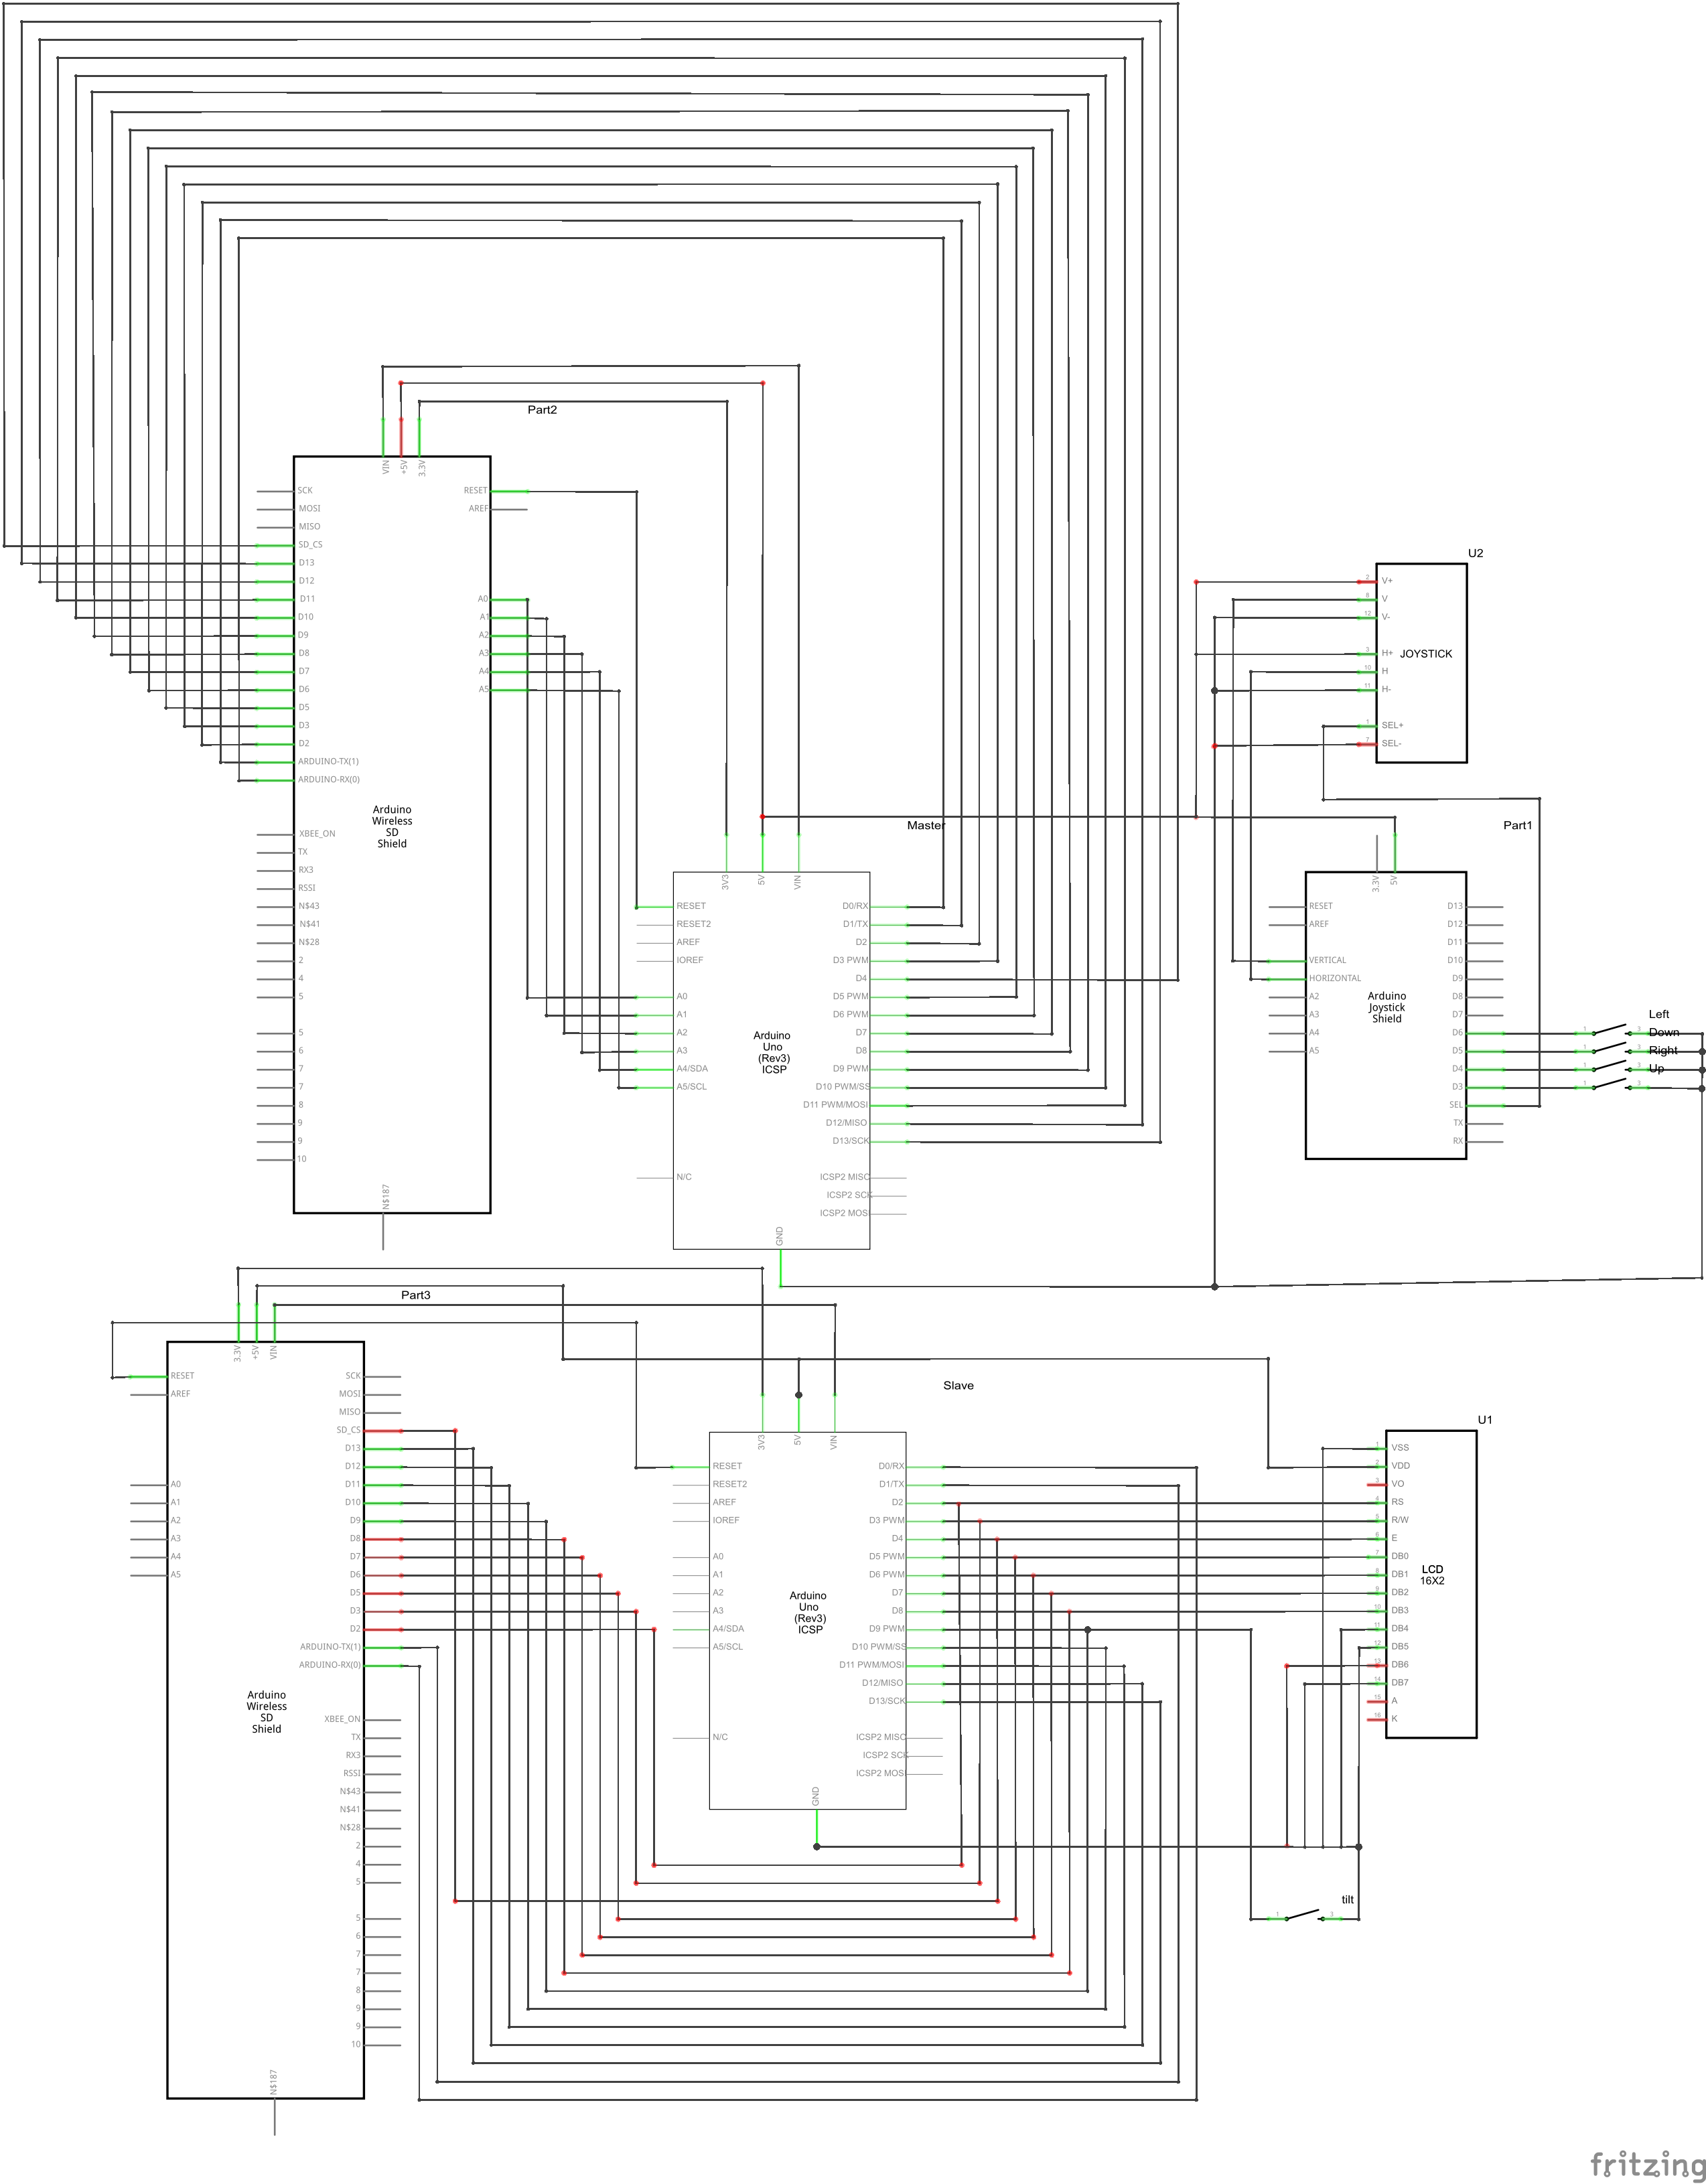
\includegraphics[width = \linewidth]{images/schem.png}
	\caption{Schematic of hardware implementation(developed using Fritzing)}
	\label{fig:schm}
\end{figure}

\subsubsection{Software Implementation}
See figure[\ref{fig:flow}].
\begin{figure}[!htbp]
	\centering
	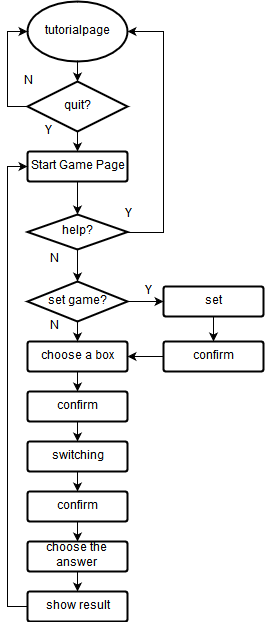
\includegraphics{images/flowchart.png}
	\caption{The flow of control}
	\label{fig:flow}
\end{figure}
	\section{TESTPLAN}
	%	Overall summary of what needs to be tested to ensure that your design meets the original requirements, 2-3 paragraphs maximum unless specified otherwise   
		We will need to test three main parts for this module. The first part is the correctness of display. The highlighted point is whether the boxes are approximately evenly distributed on the screen. The second part is the valid transmission of commands and parameters from the master board to the slave board. The highlighted point is the wireless communication and the proper setting of delay time. The wireless communication is a new thing in this lab. The basic realization is powered by XBee. We followed the instruction and set the proxies for both boards, then the two boards can communicate with an identical channel number. The third part is the control of the joystick and direction buttons. We need to test whether all the movement of the joystick can be correctly handled by the module.
	\section{PRESENTATION, DISCUSSION, AND ANALYSIS OF THE RESULTS}
	%	Based upon the execution of your design, present your results. Explain them and what was expected, and draw any conclusions (for example, did this prove your design worked).
	%	
	%	In addition to a detailed discussion and analysis of your project and your results, you must include all the answers to all questions raised in the lab.
		Since the most important part of our output is on the LCD screen, we recorded only a few screen shots of the serial monitor on PC, for the reason that the serial monitors are only used to check for the correctness of the transmission of commands. For the sake of clarity and convenience, we will show the result in the order of time, or operating logic.
\begin{figure}[!htbp]
	\centering
	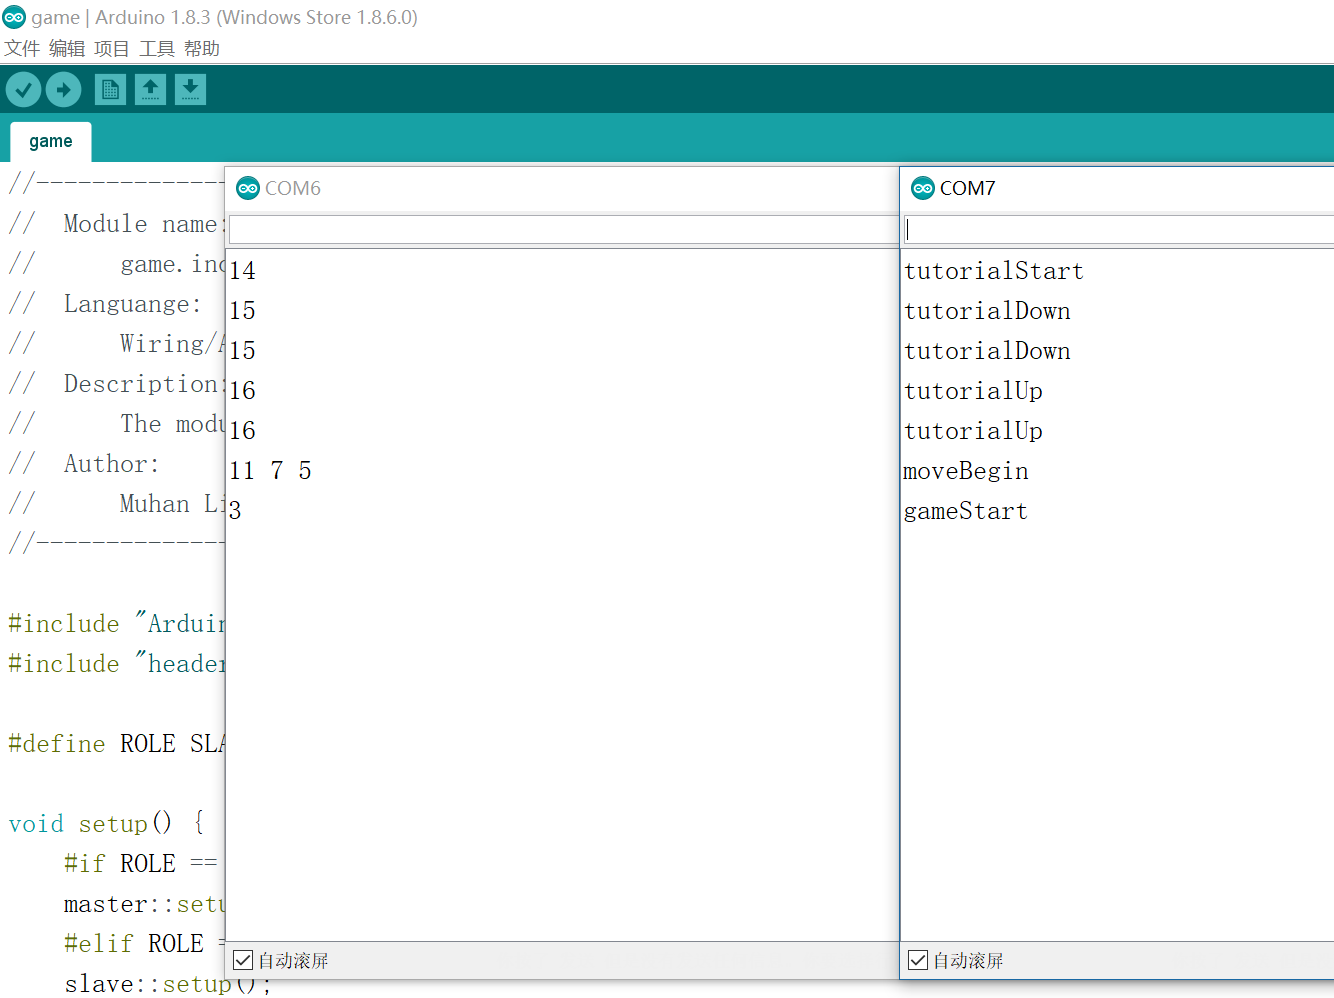
\includegraphics{images/serial.png}
	\caption{The screen shot of serial monitors before the game starts (tutorial page)}
	\label{fig:result}
\end{figure}
\paragraph{Tutorial}
We set the switch of both boards to BOARD after we loaded the modules on the corresponding boards. The serial monitor of the master board shows "14", which represents the start of the tutorial. The following commands meets with the expected results. The serial monitor of the slave board shows "tutorialStart", which indicates that the slave board receive this command and translate it correctly. More details can be found in figure[\ref{fig:result}]. Meanwhile, the LCD screen shows the first page of the tutorial pages. We move the joystick up and down to view all the pages. We push the down button or the right button to leave the tutorial pages.
\paragraph{Setting}
We push the up button to enter the setting page. We can use the joystick to move between the items and change the value of the items. We push the right button to exit the setting page and enter the start game page. In the setting page, the selected item will have left and/or right arrows around the value. The result of the display is the same as expectations.
\paragraph{Game Start}
We only need to move the joystick left and right to choose the box that we want to put something in, and start the game by pressing the right button. The number of boxes displayed on the game start page is correspondent to the number that we set in the setting page. As expected, we can use the joystick to move easily between boxes.
\paragraph{During Game}
After we pressed the right button to confirm the box we choose, the boxes will move to the middle of the screen (vertically)  and switch randomly. The speed and the time of switching depend on the speed and difficulty in the setting page. The boxes switched at an expected speed and repeated for an expected number of times. Then the boxes moved back to second line.
\paragraph{Choose Answer}
After the boxes finishing moving, we pressed the right button to start our choosing. As expected, if we choose the right box, the buzzer will play a happy melody and a heart will come out of the box. It we choose the wrong box, the buzzer will play an angry melody and a cross will come out of the box, then the right answer will be displayed. The first line of the LCD will tell us whether we win or lose. After we press the right button, a new round of game begins.
	\section{ANALYSIS OF ANY ERRORS}
	%	This one is obvious. Do this section as appropriate.  If it improves the flow, it does not need to be a separate section and may be included in the presentation, discussion, and analysis of the results.  However, it will still be graded separately and must be present.
		At first, we tried to send only the plotting command in a smaller scale through wireless communication, which means there might be at most 50 commands being sent to the slave in a second. Moreover, we should transfer the coordinates of the boxes for each command. The result was such a mess that we immediate decided that we should try another way, because it seems impossible to know what happened. Then we tried to send commands like \textit{swap a and b on the screen} instead of \textit{plot the boxes at those coordinates}. It didn't work well, but we could analyze it. What we found at last was that the reason we failed again was for the same reason as we failed before the change. The buffer of wireless communication has its limitation size. We could not send command like shooting bullets. If the slave could not read all the data in time, some incoming data would get lost. Thus, we had a few plan to fix it.
\begin{enumerate}
	\item Using a queue as a buffer. All the incoming commands are immediately read, but are handled later.
	\item Staying synchronized. The slave returns a message after finishing handling the previous command. The master should wait until it gets the message.
	\item Delay brutally. We force the master to delay a variable time based on our estimation of how long time is the slave going to take to handle the command just sent.
\end{enumerate}
\hfill \newline
We did not adopt the first plan, for the reason that it was costly to build a time sharing system in arduino. We have to check whether there are incoming commands when parsing end executing commands. We tried the second plan, but it seemed that the XBee could not support our idea. To achieve the third plan, to estimate the period each command takes, we did some calculating. The most difficult part was the moving animation. We first assumed that the time it cost had a linear relation with how many small grids it moves. Then we've got equation as follows:
\begin{equation}
	t = \lambda \times \frac{2 \times (box\_gap \times \mathrm{ceil}(LCD\_WIDTH \div num) + 2) \times 6}{2 \times speed + 1} (\mathrm{ms})
\end{equation}
\hfill \newline
We recorded period of time on various circumstances, proving that $\lambda$ was almost a constant. After several tests, we decided to have $\lambda$ as $(72+num)$, in order to avoid buffer overflow.

%	\section{ANALYSIS OF WHY THE PROJECT MAY NOT OF WORKED AND WHAT EFFORTS WERE MADE TO IDENTIFY THE ROOT CAUSE OF ANY PROBLEMS}
%	%	State any problems you encountered while working on the project. If your project did not work or worked only partially, provide an analysis of why and what efforts were made to identify the root cause of any problems. Should be written only if your project (or a required component) did not work. 
%		\input{probs}
	\section{SUMMARY AND CONCLUSIONS}
	%	You should know these sections very well, no need to explain.  Note, however, that they are two different sections.  The summary is just that, a summary of your project.  It should loosely mirror the abstract with a bit more detail.  The conclusion concludes the report, potentially adds information that is often outside the main thrust of the report, and may offer suggestions or recommendations about the project.
		\paragraph{summary}
In this report, we give a brief introduction on the purpose of the lab, a very detailed
discussion of the lab. the testplan we will apply, the result of the lab as well as its analysis, the
errors we met when doing this lab and the analysis, and the summary and conclusions of the whole
lab and report. We include a little user manual in the third section. We will also hard copy our code used in this lab to the Appendices.
\paragraph{conclusions}
We successfully designed and realized a shell game based on wireless communication, and showed our understanding of a good design.
	\section{APPENDICES}
	%	Your final version of any and all pseudocode and C code should go in this section. 
		\subsection{command.h}
\begin{minted}{c}
//----------------------------------------------------------------
//  Module name:
//      command.h
//  Languange:
//      C++
//  Description:
//      The module defines commands for xbee transfering
//  Author:
//      Man Sun, Mingxiao An
//----------------------------------------------------------------

#ifndef COMMAND_H
#define COMMAND_H

namespace command{
    void plotAnima();           // plot animation
    void choose(int);           // select one box
    void gameStart();           // the start screen
    void gameEnd();             // the end screen
    void gameOpen(int);         // open the box
    void rightOpen(int);        // open right
    void wrongOpen(int);        // open wrong
    void ready(char const*);    // display info in the first line
    void settingStart();        // prepare for the setting page
    void settingMenu(           // display a line of setting item
        int,int,int);
    void receiveEvent();        // receive a command and execute it
    void moveBegin(int,int);    // begin moving
    void moveSwap(int,int);     // swap two boxes
    void moveEnd();             // end moving
    void moveSetup(int,int);    // setting number and speed
    void tutorialStart();
    bool tutorialEnd();
    bool tutorialUp();
    bool tutorialDown();
}
#endif  // COMMAND_H
\end{minted}

\subsection{command.cpp}
\begin{minted}{c}
//----------------------------------------------------------------
//  Module name:
//      command.cpp
//  Languange:
//      C++
//  Description:
//      The module implements commands for XBee transfer
//  Author:
//      Man Sun, Mingxiao An
//----------------------------------------------------------------

#include "Arduino.h"
#include "../headers/game.h"
#include "../headers/command.h"
#include "../headers/display.h"
#include "../headers/move.h"

#define TERMINATOR '\t'

namespace command {
    int speed;
    Boxes boxes;

    enum Command {
        PLOT_ANIMA = 1,
        CHOOSE,
        GAME_START,
        GAME_END,
        GAME_OPEN = 5,
        RIGHT_OPEN,
        WRONG_OPEN,
        READY,
        SETTING_START,
        SETTING_MENU = 10,
        MOVE_BEGIN,
        MOVE_SWAP,
        MOVE_END,
        TUTORIAL_START,
        TUTORIAL_DOWN = 15,
        TUTORIAL_UP,
        TUTORIAL_END
    };

    inline void transferString(char const* str) {
        Serial.print(str);
        Serial.print(TERMINATOR);
    }

    inline void transferNum(int num) {
        Serial.print(num);
        Serial.print(' ');
    }

    inline void transferFinish() {
        Serial.print('\n');
    }

    inline void keepMoving(Boxes& boxes) {
        do {
            display::plotAnima(boxes);
            delay(20);
        } while(move::nextFrame(boxes));
    }

    inline int _step() {
        return random((speed + 1) / 2, (speed + 4) / 2);
    }

}

void command::plotAnima() {
    transferNum(Command::PLOT_ANIMA);
    transferFinish();
}

void command::choose(int boxNo) {
    transferNum(Command::CHOOSE);
    transferNum(boxNo);
    transferFinish();
}

void command::gameStart() {
    transferNum(Command::GAME_START);
    transferFinish();
}

void command::gameEnd() {
    transferNum(Command::GAME_END);
    transferFinish();
}

void command::gameOpen(int choice) {
    transferNum(Command::GAME_OPEN);
    transferNum(choice);
    transferFinish();
}

void command::rightOpen(int choice) {
    transferNum(Command::RIGHT_OPEN);
    transferNum(choice);
    transferFinish();
}

void command::wrongOpen(int choice) {
    transferNum(Command::WRONG_OPEN);
    transferNum(choice);
    transferFinish();
}

void command::ready(char const* info) {
    transferNum(Command::READY);
    transferString(info);
    transferFinish();
}

void command::settingStart() {
    transferNum(Command::SETTING_START);
    transferFinish();
}

void command::settingMenu
(int itemNo, int value, int line) {
    transferNum(Command::SETTING_MENU);
    transferNum(itemNo);
    transferNum(value);
    transferNum(line);
    transferFinish();
}

void command::moveBegin(int num, int speed) {
    transferNum(Command::MOVE_BEGIN);
    transferNum(num);
    transferNum(speed);
    transferFinish();
}

void command::moveSwap(int boxA, int boxB) {
    transferNum(Command::MOVE_SWAP);
    transferNum(boxA);
    transferNum(boxB);
    transferFinish();
}

void command::moveEnd() {
    transferNum(Command::MOVE_END);
    transferFinish();
}

void command::tutorialStart() {
    transferNum(Command::TUTORIAL_START);
    transferFinish();
}

bool command::tutorialUp() {
    transferNum(Command::TUTORIAL_UP);
    transferFinish();
    return true;
}

bool command::tutorialDown() {
    transferNum(Command::TUTORIAL_DOWN);
    transferFinish();
    return true;
}

bool command::tutorialEnd() {
    transferNum(Command::TUTORIAL_END);
    transferFinish();
    return false;
}

void command::receiveEvent() {
    int recVal0,recVal1,recVal2,recVal3;
    // char const* recStr;
    String recStr;
    bool clkws;
    Command cmd = (Command) Serial.parseInt();
    switch(cmd) {
        case Command::PLOT_ANIMA:
            Serial.println("plotAnima");
            display::plotAnima(boxes);
            break;
        case Command::CHOOSE:
            Serial.println("choose");
            recVal0 = Serial.parseInt();
            Serial.println(recVal0);
            display::choose(boxes,recVal0);
            break;
        case Command::GAME_START:
            Serial.println("gameStart");
            display::gameStart(boxes);
            break;
        case Command::GAME_END:
            move::begin(boxes);
            Serial.println("gameEnd");
            display::gameEnd(boxes);
            break;
        case Command::GAME_OPEN:
            recVal0 = Serial.parseInt();
            Serial.println("gameOpen");
            display::gameOpen(boxes,recVal0);
            break;
        case Command::RIGHT_OPEN:
            recVal0 = Serial.parseInt();
            Serial.println("rightOpen");
            display::rightOpen(boxes,recVal0);
            break;
        case Command::WRONG_OPEN:
            recVal0 = Serial.parseInt();
            Serial.println("wrongOpen");
            display::wrongOpen(boxes,recVal0);
            break;
        case Command::READY:
            // recStr = (Serial.readStringUntil(TERMINATOR)).c_str();
            recStr = Serial.readStringUntil(TERMINATOR);
            Serial.println("ready");
            Serial.println(recStr);
            display::ready(recStr);
            break;
        case Command::SETTING_START:
            display::settingStart();
            Serial.println("settingStart");
            break;
        case Command::SETTING_MENU:
            recVal0 = Serial.parseInt();
            recVal1 = Serial.parseInt();
            recVal2 = Serial.parseInt();
            Serial.println("settingMenu");
            display::settingMenu(
                script[recVal0],
                recVal1,
                _min[recVal0],
                _max[recVal0], 
                recVal2
            );
            break;
        case Command::MOVE_BEGIN:
            recVal0 = Serial.parseInt();
            boxes.num = recVal0;
            speed = Serial.parseInt();
            Serial.println("moveBegin");
            move::begin(boxes);
            keepMoving(boxes);
            break;
        case Command::MOVE_SWAP:
            recVal0 = Serial.parseInt();
            recVal1 = Serial.parseInt();
            Serial.println("moveSwap");
            clkws = random(0, 2);
            move::swap(boxes,recVal0,recVal1,clkws,_step());
            keepMoving(boxes);
            break;
        case Command::MOVE_END:
            Serial.println("moveEnd");
            move::end();
            keepMoving(boxes);
            move::begin(boxes);
            break;
        case Command::TUTORIAL_START:
            Serial.println("tutorialStart");
            display::tutorialStart();
            break;
        case Command::TUTORIAL_END:
            Serial.println("tutorialEnd");
            // display::tutorialEnd();
            break;
        case Command::TUTORIAL_UP:
            Serial.println("tutorialUp");
            display::tutorialUp();
            break;
        case Command::TUTORIAL_DOWN:
            Serial.println("tutorialDown");
            display::tutorialDown();
            break;
    }
}

\end{minted}

\subsection{constant.h}
\begin{minted}{c}
//----------------------------------------------------------------
//  Module name:
//      constant.h
//  Languange:
//      C++
//  Description:
//      The module defines global constants
//  Author:
//      Mingxiao An
//----------------------------------------------------------------

#ifndef CONSTANT_H
#define CONSTANT_H

#define MASTER 1
#define SLAVE 2
#define TEST 3

#define LCD_PORT 2, 3, 4, 5, 6, 7, 8
#define LCD_WIDTH 16
#define LCD_HEIGHT 2
#define LCD_SIZE LCD_WIDTH, LCD_HEIGHT
#define BAUD_RATE 9600

#define MAX_BOXES 8
#define MAX_CHARS 8

#define UP_PIN 2
#define RIGHT_PIN 3
#define DOWN_PIN 4
#define LEFT_PIN 5

#define SETTING_PIN UP_PIN
#define CONFIRM_PIN RIGHT_PIN
#define TUTORIAL_PIN DOWN_PIN
#define RESTART_PIN LEFT_PIN

#define X_PIN 8
#define Y_PIN 9
#define X_LEFT(x) ((x) < 256)
#define X_RIGHT(x) ((x) >= 768)
#define Y_UP(y) ((y) >= 768)
#define Y_DOWN(y) ((y) < 256)

#define NUM 0
#define SPEED 1
#define DIFFI 2

const int _min[] = {3, 1, 1};
const int _max[] = {7, 7, 7};
const char script[][11] = {
    "Box Number",
    "Move Speed",
    "Difficulty"
};

#endif  // CONSTANT_H
\end{minted}

\subsection{control.h}
\begin{minted}{c}
//----------------------------------------------------------------
//  Module name:
//      control.h
//  Languange:
//      C++
//  Description:
//      The module defines ways to attach functions to buttons
//  Author:
//      Mingxiao An
//----------------------------------------------------------------

namespace control {
    enum Position {
        UP,
        RIGHT,
        DOWN,
        LEFT
    };

    void begin();
    bool enterSettings();
    bool exitSettings();
    bool confirm();

    // return whether to continue on this attachment
    typedef bool (*callback)();

    bool nothing();
    bool confirm();

    // up, right, down, left
    void attachRod(callback, callback, callback, callback);
    void attachButton(callback, callback, callback, callback);
    // rod * 4, button * 4
    void attachPad(
        callback, callback, callback, callback, 
        callback, callback, callback, callback);
}

#define WAIT_FOR_CONFIRMING \
    control::attachButton(  \
        &control::nothing,  \
        &control::confirm,  \
        &control::nothing,  \
        &control::nothing   \
    )
\end{minted}

\subsection{control.cpp}
\begin{minted}{c}
//----------------------------------------------------------------
//  Module name:
//      control.cpp
//  Languange:
//      C++
//  Description:
//      The module implements the methods that attach functions to
//      buttons or the joystick pod
//  Author:
//      Mingxiao An
//----------------------------------------------------------------

#include "Arduino.h"
#include "../headers/constant.h"
#include "../headers/control.h"

#define UNTIL_RELEASE(pin) while (!digitalRead(pin)) delay(5)
#define UNTIL_RETURN(mode) while(mode) delay(5)

namespace control {
    bool confirm() { return false; }
    bool nothing() { return true; }
}

void control::begin() {
    pinMode(SETTING_PIN, INPUT);
    pinMode(CONFIRM_PIN, INPUT);
    pinMode(TUTORIAL_PIN, INPUT);
    pinMode(RESTART_PIN, INPUT);
    pinMode(X_PIN, INPUT);
    pinMode(Y_PIN, INPUT);
}

void control::attachButton(callback up, callback right, callback down, callback left) {
    bool flag = true;
    while (flag) {
        if (!digitalRead(UP_PIN)) {
            UNTIL_RELEASE(UP_PIN);
            flag = (*up)();
        } else if (!digitalRead(RIGHT_PIN)) {
            UNTIL_RELEASE(RIGHT_PIN);
            flag = (*right)();
        } else if (!digitalRead(DOWN_PIN)) {
            UNTIL_RELEASE(DOWN_PIN);
            flag = (*down)();
        } else if (!digitalRead(LEFT_PIN)) {
            UNTIL_RELEASE(LEFT_PIN);
            flag = (*left)();
        }
        delay(5);
    }
}

void control::attachRod(callback up, callback right, callback down, callback left) {
    bool flag = true;
    while (flag) {
        if (Y_UP(analogRead(Y_PIN))) {
            UNTIL_RETURN(Y_UP(analogRead(Y_PIN)));
            flag = (*up)();
        } else if (X_RIGHT(analogRead(X_PIN))) {
            UNTIL_RETURN(X_RIGHT(analogRead(X_PIN)));
            flag = (*right)();
        } else if (Y_DOWN(analogRead(Y_PIN))) {
            UNTIL_RETURN(Y_DOWN(analogRead(Y_PIN)));
            flag = (*down)();
        } else if (X_LEFT(analogRead(X_PIN))) {
            UNTIL_RETURN(X_LEFT(analogRead(X_PIN)));
            flag = (*left)();
        }
        delay(5);
    }
}

void control::attachPad(
    callback rodUp, callback rodRight, callback rodDown, callback rodLeft,
    callback buttonUp, callback buttonRight, callback buttonDown, callback buttonLeft) {
    bool flag = true;
    while (flag) {
        if (Y_UP(analogRead(Y_PIN))) {
            UNTIL_RETURN(Y_UP(analogRead(Y_PIN)));
            flag = (*rodUp)();
        } else if (X_RIGHT(analogRead(X_PIN))) {
            UNTIL_RETURN(X_RIGHT(analogRead(X_PIN)));
            flag = (*rodRight)();
        } else if (Y_DOWN(analogRead(Y_PIN))) {
            UNTIL_RETURN(Y_DOWN(analogRead(Y_PIN)));
            flag = (*rodDown)();
        } else if (X_LEFT(analogRead(X_PIN))) {
            UNTIL_RETURN(X_LEFT(analogRead(X_PIN)));
            flag = (*rodLeft)();
        } else if (!digitalRead(UP_PIN)) {
            UNTIL_RELEASE(UP_PIN);
            flag = (*buttonUp)();
        } else if (!digitalRead(RIGHT_PIN)) {
            UNTIL_RELEASE(RIGHT_PIN);
            flag = (*buttonRight)();
        } else if (!digitalRead(DOWN_PIN)) {
            UNTIL_RELEASE(DOWN_PIN);
            flag = (*buttonDown)();
        } else if (!digitalRead(LEFT_PIN)) {
            UNTIL_RELEASE(LEFT_PIN);
            flag = (*buttonLeft)();
        }
        delay(5);
    }
}
\end{minted}

\subsection{display.h}
\begin{minted}{c}
//----------------------------------------------------------------
//  Module name:
//      display.h
//  Languange:
//      C++
//  Description:
//      The module defines display methods
//  Author:
//      Mingxiao An, Man Sun
//----------------------------------------------------------------

#ifndef DISPLAY_H
#define DISPLAY_H

#include "game.h"
#include "Arduino.h"

namespace display {
    void clear();
    void begin();               // initialize lcd
    void plotAnima(Boxes&);     // plot animation
    void choose(Boxes&, int);   // select one box
    void gameStart(Boxes&);     // the start screen
    void gameEnd(Boxes&);       // the end screen
    void gameOpen(Boxes&, int); // open the box
    void rightOpen(Boxes&, int);// open right
    void wrongOpen(Boxes&, int);// open wrong
    void ready(char const*);    // display info in the first line
    void ready(String&);
    void settingStart();        // prepare for the setting page
    void settingMenu(           // display a line of setting item
        char const*,int,int,int,int);
    void tutorialStart();
    void tutorialUp();
    void tutorialDown();
}

#endif  // DISPLAY_H

\end{minted}

\subsection{display.cpp}
\begin{minted}{c}
//----------------------------------------------------------------
//  Module name:
//      display.cpp
//  Languange:
//      C++
//  Description:
//      The module inplements display methods
//  Author:
//      Mingxiao An, Man Sun
//----------------------------------------------------------------

#include "Arduino.h"
#include <LiquidCrystal.h>
#include "../headers/display.h"
#include "../headers/game.h"
#include "../headers/graph.h"
#include "../headers/sound.h"

#define EACH_COL(i) (int i = 0; i < LCD_WIDTH; i ++)
#define EACH_ROW(i) (int i = 0; i < LCD_HEIGHT; i ++)
#define EACH_BOX(i) (int i = 0; i < boxes.num; i ++)

#define LEFTARROW (char)0
#define RIGHTARROW (char)1
#define BOX (char)2
#define OPENBOX (char)3
#define OPENRIGHT (char)4
#define OPENWRONG (char)5
#define BRACKETL (char)6
#define BRACKETR (char)7

namespace display {

    LiquidCrystal *lcd;
    Map display[LCD_WIDTH][LCD_HEIGHT];
    Char charList[MAX_CHARS];
    int charListIndex;
    int tutorialLine;

    inline int _inCharList(Char ch) {
        for (int i = 0; i < charListIndex; i ++) {
            if (charList[i] == ch) {
                return i;
            }
        }
        return charListIndex;
    }

    inline int _gridCol(int col) {
        return col * 6 - 2;
    }

    inline int _gridRow(int row) {
        return row * 9 - 2;
    }

    inline int _gridColCenter(int col) {
        return col * 6 + 2;
    }

    inline int _gridRowCenter(int row) {
        return row == 0 ? 2: 14;
    }

    void _initDisplay() {
        for EACH_COL(i) {
            for EACH_ROW(j) {
                display[i][j].smap = ' ';
            }
        }
    }

    void _refreshDisplay() {
        for (int i = 0; i < charListIndex; i ++) {
            lcd->createChar(i, charList[i]);
        }
        lcd->setCursor(0, 0);
        for EACH_COL(i) {
            lcd->print(display[i][0].smap);
        }
        lcd->setCursor(0, 1);
        for EACH_COL(i) {
            lcd->print(display[i][1].smap);
        }
    }
}

void display::clear() {
    lcd->clear();
}

void display::begin() {
    lcd = new LiquidCrystal(LCD_PORT);
    lcd->begin(LCD_SIZE);
    _initDisplay();
    _refreshDisplay();
}

void display::plotAnima(Boxes& boxes) {
    charListIndex = 0;
    charList[charListIndex++] = bitmaps[VERTICAL][1];
    charList[charListIndex++] = bitmaps[VERTICAL][10];

    for EACH_COL(i) {
        for EACH_ROW(j) {
            int gridCol = _gridCol(i);
            int gridColCenter = _gridColCenter(i);
            int gridRow = _gridRow(j);
            int gridRowCenter = _gridRowCenter(j);
            int col_relative = -1;
            int row_relative = -1;

            for EACH_BOX(k) {
                // same row first, same col second
                if (boxes.pos[k].r == gridRowCenter) {
                    int _relative = boxes.pos[k].c - gridCol;
                    if (_relative >= 0 && _relative < 9)
                        col_relative = _relative;
                } else if (boxes.pos[k].c == gridColCenter) {
                    int _relative = boxes.pos[k].r - gridRow;
                    if (_relative >= 0 && _relative < 12)
                        row_relative = _relative;
                }
            }

            if (col_relative == -1 && row_relative == -1) { // neither same row or col
                display[i][j].map = NULL;
                display[i][j].smap = ' ';
            } else {
                if (col_relative == -1) {                   // same col without same row
                    display[i][j].map = bitmaps[VERTICAL][row_relative];
                } else {
                    if (row_relative == -1) {               // same row without same col
                        display[i][j].map = bitmaps[
                            j == 0 ? HORIZONTAL_LINE1 : HORIZONTAL_LINE2
                        ][col_relative];
                    } else {                                // both same row and col
                        display[i][j].map = bitmaps[
                            j == 0 ? HORIZONTAL_LINE1_WITH: HORIZONTAL_LINE2_WITH
                        ][col_relative];
                    }
                }
                // insert the char to the list if it is a new char
                display[i][j].smap = (char)_inCharList(display[i][j].map);
                if (display[i][j].smap == (char)charListIndex) {
                    charList[charListIndex++] = display[i][j].map;
                }
            }
        }
    }

    _refreshDisplay();
}

void display::choose(Boxes& boxes, int select) {
    for EACH_BOX(i) {
        int col = boxes.pos[i].c / 6;
        lcd->setCursor(col - 1, 1);
        lcd->print(' ');
        lcd->setCursor(col + 1, 1);
        lcd->print(' ');
    }
    int col = boxes.pos[select].c / 6;
    lcd->setCursor(col - 1, 1);
    lcd->print(BRACKETL);
    lcd->setCursor(col + 1, 1);
    lcd->print(BRACKETR);
}

void display::ready(char const *s) {
    lcd->setCursor(0, 0);
    lcd->print("                ");
    lcd->setCursor(0, 0);
    lcd->print(s);
}

void display::ready(String& s) {
    lcd->setCursor(0, 0);
    lcd->print("                ");
    lcd->setCursor(0, 0);
    lcd->print(s);
}

void display::gameStart(Boxes& boxes) {
    lcd->clear();
    lcd->createChar(BOX, box);
    lcd->createChar(BRACKETL, bracketL);
    lcd->createChar(BRACKETR, bracketR);
    for EACH_BOX(i) {
        int col = boxes.pos[i].c / 6;
        lcd->setCursor(col, 1);
        lcd->print(BOX);
    }
    choose(boxes, 0);
    ready("Choose to start:");
}

void display::gameEnd(Boxes& boxes) {
    lcd->createChar(BOX, box);
    lcd->createChar(OPENBOX, openBox);
    lcd->createChar(OPENRIGHT, openRight);
    lcd->createChar(OPENWRONG, openWrong);
    lcd->createChar(BRACKETL, bracketL);
    lcd->createChar(BRACKETR, bracketR);
    for EACH_BOX(i) {
        int col = boxes.pos[i].c / 6;
        lcd->setCursor(col, 1);
        lcd->print(BOX);
    }
    choose(boxes, 0);
    ready("Choose your box:");
}

void display::gameOpen(Boxes& boxes, int select) {
    int col = boxes.pos[select].c / 6;
    lcd->setCursor(col, 1);
    lcd->print(OPENBOX);
}

void display::rightOpen(Boxes& boxes, int select) {
    int col = boxes.pos[select].c / 6;
    lcd->setCursor(col, 0);
    lcd->print(OPENRIGHT);
    lcd->setCursor(col-1,1);
    lcd->print(' ');
    lcd->setCursor(col+1,1);
    lcd->print(' ');
    soundSuccess();
}

void display::wrongOpen(Boxes& boxes, int select) {
    int col = boxes.pos[select].c / 6;
    lcd->setCursor(col, 0);
    lcd->print(OPENWRONG);
    lcd->setCursor(col-1,1);
    lcd->print(' ');
    lcd->setCursor(col+1,1);
    lcd->print(' ');
    soundWA();
}

void display::settingStart() {
    lcd->clear();
    lcd->createChar(LEFTARROW,leftArrow);
    lcd->createChar(RIGHTARROW,rightArrow);
}

void display::settingMenu
(char const* item, int value, int min, int max, int line) {
    lcd->setCursor(0,line);
    lcd->print(item);
    lcd->print("   ");
    if(min < value) lcd->print(LEFTARROW);
    else lcd->print(" ");
    lcd->print(value);
    if(max > value) lcd->print(RIGHTARROW);
    else lcd->print(" ");

    if (line == 1) line = 0;
    else line = 1;
    lcd->setCursor(13, line);
    lcd->print(" ");
    lcd->setCursor(15, line);
    lcd->print(" ");
}

void display::tutorialStart() {
    lcd->clear();
    tutorialLine = 0;
    lcd->print(tutorialLine1);
    lcd->setCursor(0, 1);
    lcd->print(tutorialLine2);
}

void display::tutorialUp() {
    switch (tutorialLine) {
        case 1:
            lcd->setCursor(0, 0);
            lcd->print(tutorialLine1);
            lcd->setCursor(0, 1);
            lcd->print(tutorialLine2);
            tutorialLine -= 1;
            break;
        case 2:
            lcd->setCursor(0, 0);
            lcd->print(tutorialLine2);
            lcd->setCursor(0, 1);
            lcd->print(tutorialLine3);
            tutorialLine -= 1;
            break;      
    }
}

void display::tutorialDown() {
    switch (tutorialLine) {
        case 0:
            lcd->setCursor(0, 0);
            lcd->print(tutorialLine2);
            lcd->setCursor(0, 1);
            lcd->print(tutorialLine3);
            tutorialLine += 1;
            break;
        case 1:
            lcd->setCursor(0, 0);
            lcd->print(tutorialLine3);
            lcd->setCursor(0, 1);
            lcd->print(tutorialLine4);
            tutorialLine += 1;
            break;
    }
}
\end{minted}

\subsection{game.h}
\begin{minted}{c}
//----------------------------------------------------------------
//  Module name:
//      game.h
//  Languange:
//      C++
//  Description:
//      The module defines basic game-control-related design
//  Author:
//      Mingxiao An
//----------------------------------------------------------------

#ifndef GAME_H
#define GAME_H

#include "constant.h"

struct Pos {
    int c, r;   // column and row in micro grid
};

struct Boxes {
    int num;
    Pos pos[MAX_BOXES];
};

typedef unsigned char *Char;

struct Map {
    char smap;  // the lcd mapping
    Char map;   // the global mapping
};

namespace game {
    void newGame();
    void setting();
    void tutorial();
}

namespace master {
    void setup();
    void loop();
}

namespace slave {
    void setup();
    void loop();
}

namespace test {
    void setup();
    void loop();
}

#endif  // GAME_H
\end{minted}

\subsection{game.cpp}
\begin{minted}{c}
//----------------------------------------------------------------
//  Module name:
//      game.cpp
//  Languange:
//      C++
//  Description:
//      The module implements game, setting, and tutorial control
//  Author:
//      Mingxiao An, Man Sun
//----------------------------------------------------------------

#include "Arduino.h"
#include "../headers/game.h"
#include "../headers/command.h"
#include "../headers/control.h"

#define RANDOM_CLOCKWIZE random(0, 2)

#define NUM 0
#define SPEED 1
#define DIFFI 2
#define SETTING_MENU(x, l) command::settingMenu(x, *settings[x], l)

namespace game {

    int num = 7;    // number of boxes
    int speed = 5;  // the speed level
                    // minspeed = (speed + 1) / 2
                    // maxspeed = (speed + 4) / 2
    int diffi = 1;  // the times of moving = 5 * diffi + 5
    int choice = 0;
    int select = 0;
    int settingLine = NUM;
    int cursorLine = 0;

    int *settings[] = {&num, &speed, &diffi};

    inline int _step() {
        return random((speed + 1) / 2, (speed + 4) / 2);
    }

    bool chooseLeft() {
        if (choice != 0) {
            choice -= 1;
            command::choose(choice);
        }
        return true;
    }

    bool chooseRight() {
        if (choice != num - 1) {
            choice += 1;
            command::choose(choice);
        }
        return true;
    }

    bool selectLeft() {
        if (select != 0) {
            select -= 1;
            command::choose(select);
        }
        return true;
    }

    bool selectRight() {
        if (select != num - 1) {
            select += 1;
            command::choose(select);
        }
        return true;
    }

    bool goToSetting() {
        setting();
        return true;
    }

    bool settingUp() {
        switch (settingLine) {
            case 0: 
                break;
            case 1: 
                settingLine -= 1;
                SETTING_MENU(1, 1);
                SETTING_MENU(0, 0);
                break;
            case 2:
                settingLine -= 1;
                SETTING_MENU(2, 1);
                SETTING_MENU(1, 0);
                break;
        }
        cursorLine = 0;
        return true;
    }

    bool settingDown() {
        switch (settingLine) {
            case 0: 
                settingLine += 1;
                SETTING_MENU(0, 0);
                SETTING_MENU(1, 1);
                break;
            case 1: 
                settingLine += 1; 
                SETTING_MENU(1, 0);
                SETTING_MENU(2, 1);
                break;
            case 2:
                break;
        }
        cursorLine = 1;
        return true;
    }

    bool settingRight() {
        if (*settings[settingLine] < _max[settingLine]) {
            *settings[settingLine] += 1;
            SETTING_MENU(settingLine, cursorLine);
        }
        return true;
    }

    bool settingLeft() {
        if (*settings[settingLine] > _min[settingLine]) {
            *settings[settingLine] -= 1;
            SETTING_MENU(settingLine, cursorLine);
        }
        return true;
    }

    bool goToTutorial() {
        tutorial();
        return true;
    }
}

using control::nothing;
using control::confirm;

void game::newGame() {
    command::moveBegin(num,speed);
    choice = 0;
    command::gameStart();
    delay(1000);
    // command::choose(choice);
    control::attachPad(
        &nothing, &chooseRight, &nothing, &chooseLeft, 
        &goToSetting, &confirm, &goToTutorial, &nothing
    );

    command::ready("3");
    delay(1000);
    command::ready("2");
    delay(1000);
    command::ready("1");
    delay(1000);
    command::ready("Go");
    delay(500);

    command::moveBegin(num, speed);
    for(int i = 5 * diffi + 5; i > 0; i --) {
        // generate random 2 boxes
        int box1 = random(0, num);
        int box2 = random(1, num);
        if (box2 == box1) {
            box2 = 0;
        }
        if (box1 == choice) {
            choice = box2;
        } else if (box2 == choice) {
            choice = box1;
        }
        command::moveSwap(box1,box2);
        int gap = box1 - box2;
        if (gap < 0) gap = -gap;
        int delayTime = (2 * gap * (LCD_WIDTH / num) + 2) * 6 * (72 + diffi) / (2 * speed + 1);
        delay(delayTime);
    }
    command::moveEnd();

    // move::begin(boxes);
    // display::plotAnima(boxes);
    // DELAY;
    // while (move::nextFrame(boxes)) {
    //  display::plotAnima(boxes);
    //  DELAY;
    // }
    // for (int i = 5 * diffi + 5; i > 0; i --) {
    //  // generate random 2 boxes
    //  int box1 = random(0, num);
    //  int box2 = random(1, num);
    //  if (box2 == box1) {
    //      box2 = 0;
    //  }
    //  if (box1 == choice) {
    //      choice = box2;
    //  } else if (box2 == choice) {
    //      choice = box1;
    //  }
    //  move::swap(
    //      boxes, box1, box2, 
    //      RANDOM_CLOCKWIZE,
    //      _step()
    //  );
    //  while (move::nextFrame(boxes)) {
    //      display::plotAnima(boxes);
    //      DELAY;
    //  }
    // }
    // move::end();
    // while (move::nextFrame(boxes)) {
    //  display::plotAnima(boxes);
    //  DELAY;
    // }

    WAIT_FOR_CONFIRMING;
    select = 0;
    command::gameEnd();

    control::attachPad(
        &nothing, &selectRight, &nothing, &selectLeft, 
        &nothing, &confirm, &nothing, &nothing
    );

    command::gameOpen(select);
    delay(1000);
    command::ready("");
    if (choice == select) {
        command::rightOpen(select);
        delay(1000);
        command::ready("You Win! :)");
    } else {
        command::wrongOpen(select);
        delay(1000);
        command::ready("You Lose! :(");
        WAIT_FOR_CONFIRMING;
        command::ready("The answer is:");
        delay(1000);
        command::gameOpen(choice);
        delay(1000);
        command::ready("");
        command::rightOpen(choice);
    }
    
    WAIT_FOR_CONFIRMING;
}

void game::setting() {
    settingLine = NUM;
    cursorLine = 0;
    command::settingStart();
    SETTING_MENU(SPEED, 1);
    SETTING_MENU(NUM, 0);
    control::attachPad(
        &settingUp,
        &settingRight,
        &settingDown,
        &settingLeft,
        &confirm,
        &confirm,
        &nothing,
        &nothing
    );
    command::moveBegin(num,speed);
    choice = 0;
    command::gameStart();
}

void game::tutorial() {
    command::tutorialStart();
    control::attachPad(
        &command::tutorialUp,
        &nothing,
        &command::tutorialDown,
        &nothing,
        &nothing,
        &confirm,
        &confirm,
        &nothing
    );
    command::moveBegin(num, speed);
    choice = 0;
    command::gameStart();
}
\end{minted}

\subsection{game.ino}
\begin{minted}{c}
//----------------------------------------------------------------
//  Module name:
//      game.ino
//  Languange:
//      Wiring/Arduino
//  Description:
//      The module is the top module of the shell game
//  Author:
//      Muhan Li
//----------------------------------------------------------------

#include "Arduino.h"
#include "headers/game.h"

#define ROLE SLAVE

void setup() {
    #if ROLE == MASTER
    master::setup();
    #elif ROLE == SLAVE
    slave::setup();
    #elif ROLE == TEST
    test::setup();
    #endif  // ROLE
}

void loop() {
    #if ROLE == MASTER
    master::loop();
    #elif ROLE == SLAVE
    slave::loop();
    #elif ROLE == TEST
    test::loop();
    #endif  // ROLE
}
\end{minted}

\subsection{master.cpp}
\begin{minted}{c}
//----------------------------------------------------------------
//  Module name:
//      master.cpp
//  Languange:
//      C++
//  Description:
//      The module implements the master's behavior
//  Author:
//      Muhan Li
//----------------------------------------------------------------

#include "Arduino.h"
#include "../headers/game.h"
#include "../headers/control.h"

void master::setup() {
    Serial.begin(BAUD_RATE);
    control::begin();
    randomSeed(analogRead(12));
    game::tutorial();
}

void master::loop() {
    game::newGame();
}
\end{minted}

\subsection{move.h}
\begin{minted}{c}
//----------------------------------------------------------------
//  Module name:
//      move.h
//  Languange:
//      C++
//  Description:
//      The module defines coordinate computing methods for 
//      moving boxes
//  Author:
//      Man Sun
//----------------------------------------------------------------

#ifndef MOVE_H
#define MOVE_H

#include "game.h"

namespace move {
    void swap(Boxes&,int boxA, int boxB, bool clockwise, int step);
    void begin(Boxes&);
    void end();
    bool nextFrame(Boxes&);
}

#endif  // MOVE_H
\end{minted}

\subsection{move.cpp}
\begin{minted}{c}
//----------------------------------------------------------------
//  Module name:
//      move.cpp
//  Languange:
//      C++
//  Description:
//      The module implements coordinate computing methods for 
//      moving boxes
//  Author:
//      Man Sun
//----------------------------------------------------------------

#ifndef MOVE_H
#define MOVE_H

#include "game.h"

namespace move {
    void swap(Boxes&,int boxA, int boxB, bool clockwise, int step);
    void begin(Boxes&);
    void end();
    bool nextFrame(Boxes&);
}

#endif  // MOVE_H
#include "../headers/game.h"
#include "../headers/move.h"

#define BLOCKWIDTH 6
#define BLOCKHEIGHT 8
#define LCDWIDTH 16
#define LCDHEIGHT 2
#define BEGINFRAMES 4
#define BEGINHEIGHT 13
#define ENDFRAMES 4
#define MOVEVERSTEPS 6
#define TOPROW 2
#define BOTTOMROW 14
#define LEFTCOL 2
#define RIGHTCOL 92

namespace move {
    enum phase {BEGIN, SWITCH_OUT, SWITCH_HOR, SWITCH_BAK, END} crtPhase;
    int stepLen;
    int stepsRemain;
    int switchBoxL, switchBoxR;
    bool switchClockwise;
    int blocksBetweenBox;

    // change the number(start from 1) of the block to the column of its central bit(start from 0)
    int block2col(int blockCol) {
        return (BLOCKWIDTH * blockCol - BLOCKWIDTH/2 - 1);
    }

    // get the column of the central bit of the certain box
    int getCol(Boxes &boxes, int boxNo) {
        return (boxes.pos[boxNo].c);
    }

    // get the row of the central bit of the certain box
    int getRow(Boxes &boxes, int boxNo) {
        return (boxes.pos[boxNo].r);
    }

    // set the column of the central bit of the certain box
    void setCol(Boxes &boxes, int boxNo, int col) {
        if(col < LEFTCOL || col > RIGHTCOL) return;
        boxes.pos[boxNo].c = col;
    }

    // set the row of the central bit of the certain box
    void setRow(Boxes &boxes, int boxNo, int row) {
        if(row < TOPROW || row > BOTTOMROW) return;
        boxes.pos[boxNo].r = row;
    }

    // move the certain box down by step bit(s)
    void moveDown(Boxes &boxes, int boxNo, int step = 1) {
        if(getRow(boxes,boxNo) == BOTTOMROW) return;
        if(getRow(boxes,boxNo) + step > BOTTOMROW) setRow(boxes,boxNo,BOTTOMROW);
        else boxes.pos[boxNo].r += step;
    }

    // move the certain box up by step bit(s)
    void moveUp(Boxes &boxes, int boxNo, int step = 1) {
        if(getRow(boxes,boxNo) == TOPROW) return;
        if(getRow(boxes,boxNo) - step < TOPROW) setRow(boxes,boxNo,TOPROW);
        else boxes.pos[boxNo].r -= step;
    }

    // move the certain box left by step bit(s)
    void moveLeft(Boxes &boxes, int boxNo, int step = 1) {
        if(getCol(boxes,boxNo) == LEFTCOL) return;
        if(getCol(boxes,boxNo) - step < LEFTCOL) setCol(boxes,boxNo,LEFTCOL);
        else boxes.pos[boxNo].c -= step;
    }

    // move the certain box right by step bit(s)
    void moveRight(Boxes &boxes, int boxNo, int step = 1) {
        if(getCol(boxes,boxNo) == RIGHTCOL) return;
        if(getCol(boxes,boxNo) + step > RIGHTCOL) setCol(boxes,boxNo,RIGHTCOL);
        else boxes.pos[boxNo].c += step;
    }

    // set all the box in boxes to the central from left to right
    void initPos(Boxes &boxes)
    {
        int margin = (LCDWIDTH - boxes.num - blocksBetweenBox * (boxes.num - 1)) / 2;
        for(int i = 0;i<boxes.num;i++)
        {   
            int crtCol = block2col(margin + i * (blocksBetweenBox + 1) + 2);
            setCol(boxes,i,crtCol);
            setRow(boxes,i,BLOCKHEIGHT);
        }
    }

    // move all the boxes up for 1 bit
    void beginMove(Boxes &boxes) {
        for(int i = 0;i<boxes.num;i++) {
            moveUp(boxes,i);
        }
    }

    // move the two swapped boxes out of the queue by 1 bit according to the direction
    void switchOut(Boxes &boxes) {
        if(switchClockwise) {
            moveUp(boxes,switchBoxL,stepLen);
            moveDown(boxes,switchBoxR,stepLen);
        } else {
            moveUp(boxes,switchBoxR,stepLen);
            moveDown(boxes,switchBoxL,stepLen);
        }

        if(getRow(boxes,switchBoxL) == (switchClockwise ? TOPROW : BOTTOMROW)) {
            stepsRemain = (switchBoxR - switchBoxL) * (blocksBetweenBox + 1) * BLOCKWIDTH;
            stepsRemain = (stepsRemain + stepLen - 1) / stepLen;
            crtPhase = SWITCH_HOR;
        }
    }

    // move the two swapped boxes horizontally by 1 bit according to the direction
    void switchHorizontal(Boxes &boxes) {
        if(switchClockwise) {
            moveRight(boxes,switchBoxL,stepLen);
            moveLeft(boxes,switchBoxR,stepLen);
        } else {
            moveRight(boxes,switchBoxL,stepLen);
            moveLeft(boxes,switchBoxR,stepLen);
        }

        if(stepsRemain == 0) {
            stepsRemain = MOVEVERSTEPS;
            stepsRemain = (stepsRemain + stepLen - 1) / stepLen;
            crtPhase = SWITCH_BAK;
        }
    }

    // move the two swapped boxes back to the queue by 1 bit according to the direction
    void switchBack(Boxes &boxes) {
        if(switchClockwise) {
            moveDown(boxes,switchBoxL,stepLen);
            moveUp(boxes,switchBoxR,stepLen);
        } else {
            moveDown(boxes,switchBoxR,stepLen);
            moveUp(boxes,switchBoxL,stepLen);
        }
    }

    // move all the boxes down by 1 bit
    void endMove(Boxes &boxes) {
        for(int i = 0;i<boxes.num;i++) {
            moveDown(boxes,i);
        }
    }
    
}



// set all the boxes to their beginning positions
void move::begin(Boxes &boxes) {
    crtPhase = BEGIN;
    stepsRemain = BEGINFRAMES;
    blocksBetweenBox = LCDWIDTH / boxes.num - 1;
    int margin = (LCDWIDTH - boxes.num - blocksBetweenBox * (boxes.num - 1)) / 2;
    for(int i = 0;i<boxes.num;i++)
    {   
        int crtCol = block2col(margin + i * (blocksBetweenBox + 1) + 2);
        setCol(boxes,i,crtCol);
        setRow(boxes,i,BEGINHEIGHT);
    }
}

// record the number of the two swapped boxes and the direction
void move::swap(Boxes &boxes, int boxA, int boxB, bool clockwise,int step) {
    crtPhase = SWITCH_OUT;
    initPos(boxes);
    if (boxA < boxB) {
        switchBoxL = boxA;
        switchBoxR = boxB;
    } else {
        switchBoxL = boxB;
        switchBoxR = boxA;
    }
    switchClockwise = clockwise;
    stepLen = step;

    stepsRemain = MOVEVERSTEPS;
    stepsRemain = (stepsRemain + stepLen - 1) / stepLen;
}

// set all the boxes to their ending positions
void move::end() {
    crtPhase = END;
    stepsRemain = ENDFRAMES;
}

// modify the current positions according to the phases and remaining steps
// return true if there are still remaining steps, false if not
bool move::nextFrame(Boxes &boxes) {
    if(stepsRemain == 0) return false;
    else stepsRemain -= 1;
    switch(crtPhase) {
        case BEGIN:
            beginMove(boxes);
            break;
        case SWITCH_OUT:
            switchOut(boxes);
            break;
        case SWITCH_HOR:
            switchHorizontal(boxes);
            break;
        case SWITCH_BAK:
            switchBack(boxes);
            break;
        case END:
            endMove(boxes);
            break;
    }
    return true;
}
\end{minted}

\subsection{pitches.h}
\begin{minted}{c}
//----------------------------------------------------------------
//  Module name:
//      pitches.h
//  Languange:
//      C++
//  Description:
//      The module defines constants of pitches
//  Author:
//      Muhan Li
//----------------------------------------------------------------

/*************************************************
 * Public Constants
 *************************************************/

#define NOTE_B0  31
#define NOTE_C1  33
#define NOTE_CS1 35
#define NOTE_D1  37
#define NOTE_DS1 39
#define NOTE_E1  41
#define NOTE_F1  44
#define NOTE_FS1 46
#define NOTE_G1  49
#define NOTE_GS1 52
#define NOTE_A1  55
#define NOTE_AS1 58
#define NOTE_B1  62
#define NOTE_C2  65
#define NOTE_CS2 69
#define NOTE_D2  73
#define NOTE_DS2 78
#define NOTE_E2  82
#define NOTE_F2  87
#define NOTE_FS2 93
#define NOTE_G2  98
#define NOTE_GS2 104
#define NOTE_A2  110
#define NOTE_AS2 117
#define NOTE_B2  123
#define NOTE_C3  131
#define NOTE_CS3 139
#define NOTE_D3  147
#define NOTE_DS3 156
#define NOTE_E3  165
#define NOTE_F3  175
#define NOTE_FS3 185
#define NOTE_G3  196
#define NOTE_GS3 208
#define NOTE_A3  220
#define NOTE_AS3 233
#define NOTE_B3  247
#define NOTE_C4  262
#define NOTE_CS4 277
#define NOTE_D4  294
#define NOTE_DS4 311
#define NOTE_E4  330
#define NOTE_F4  349
#define NOTE_FS4 370
#define NOTE_G4  392
#define NOTE_GS4 415
#define NOTE_A4  440
#define NOTE_AS4 466
#define NOTE_B4  494
#define NOTE_C5  523
#define NOTE_CS5 554
#define NOTE_D5  587
#define NOTE_DS5 622
#define NOTE_E5  659
#define NOTE_F5  698
#define NOTE_FS5 740
#define NOTE_G5  784
#define NOTE_GS5 831
#define NOTE_A5  880
#define NOTE_AS5 932
#define NOTE_B5  988
#define NOTE_C6  1047
#define NOTE_CS6 1109
#define NOTE_D6  1175
#define NOTE_DS6 1245
#define NOTE_E6  1319
#define NOTE_F6  1397
#define NOTE_FS6 1480
#define NOTE_G6  1568
#define NOTE_GS6 1661
#define NOTE_A6  1760
#define NOTE_AS6 1865
#define NOTE_B6  1976
#define NOTE_C7  2093
#define NOTE_CS7 2217
#define NOTE_D7  2349
#define NOTE_DS7 2489
#define NOTE_E7  2637
#define NOTE_F7  2794
#define NOTE_FS7 2960
#define NOTE_G7  3136
#define NOTE_GS7 3322
#define NOTE_A7  3520
#define NOTE_AS7 3729
#define NOTE_B7  3951
#define NOTE_C8  4186
#define NOTE_CS8 4435
#define NOTE_D8  4699
#define NOTE_DS8 4978
\end{minted}

\subsection{slave.cpp}
\begin{minted}{c}
//----------------------------------------------------------------
//  Module name:
//      slave.cpp
//  Languange:
//      C++
//  Description:
//      The module implements the slave's behavior
//  Author:
//      Muhan Li
//----------------------------------------------------------------

#include "Arduino.h"
#include "../headers/game.h"
#include "../headers/command.h"
#include "../headers/display.h"

#define TILT 11
#define BUZZER 9

void slave::setup() {
    pinMode(BUZZER, OUTPUT);
    display::begin();
    Serial.begin(BAUD_RATE);
    randomSeed(analogRead(12));
}

void slave::loop() {
    if (Serial.available() > 0) {
        command::receiveEvent();
    }
    if (!digitalRead(TILT)) {
        display::clear();
    }
}
\end{minted}

\subsection{sound.h}
\begin{minted}{c}
//----------------------------------------------------------------
//  Module name:
//      sound.h
//  Languange:
//      C++
//  Description:
//      The module defines and implements sound effects for buzzer
//  Author:
//      Muhan Li
//----------------------------------------------------------------

#ifndef SOUND_H
#define SOUND_H
#define BUZZER_PORT 9

#include "pitches.h"

int melody[][5] = {
    { NOTE_C5, NOTE_E5, NOTE_G5, NOTE_E5, NOTE_G5 },
    { NOTE_G3, NOTE_G3 }
};

int noteDuration[][5]{
    { 375, 125, 375, 125, 1000 },
    { 500, 1500 }
};

void soundSuccess() {
    for (int i = 0; i < 5; i++) {
        tone(BUZZER_PORT, melody[0][i], noteDuration[0][i]);
        delay(noteDuration[0][i] * 1.30);
    }
}

void soundWA() {
    for (int i = 0; i < 2; i++) {
        tone(BUZZER_PORT, melody[1][i], noteDuration[1][i]);
        delay(noteDuration[1][i] * 1.30);
    }
}

#endif
\end{minted}

\subsection{test.cpp}
\begin{minted}{c}
//----------------------------------------------------------------
//  Module name:
//      test.cpp
//  Languange:
//      C++
//  Description:
//      The module is for testing
//  Author:
//      Muhan Li, Man Sun, Mingxiao An
//----------------------------------------------------------------

#include "Arduino.h"
#include "../headers/display.h"
#include "../headers/move.h"
#include "../headers/control.h"
#include "../headers/game.h"

bool _up() {
    Serial.println("up");
    return true;
}

bool _right() {
    Serial.println("right");
    return false;
}

bool _down() {
    Serial.println("down");
    return true;
}

bool _left() {
    Serial.println("left");
    return true;
}

void test::setup() {
    Serial.begin(BAUD_RATE);
    control::begin();
}

void test::loop() {
    Serial.println("Start one");
    control::attachButton(&_up, &_right, &_down, &_left);
    Serial.println("Finish one");
}
\end{minted}

\subsection{graph.h}
\begin{minted}{c}
//----------------------------------------------------------------
//  Module name:
//      graph.h
//  Languange:
//      C++
//  Description:
//      The module defines character bitmaps to show on lcd
//  Author:
//      Man Sun, Muhan Li
//----------------------------------------------------------------

#ifndef GRAPH_H
#define GRAPH_H

#include "Arduino.h"

// category: 0 for vertical, line: 1,2
// category: 1 for horizontal with one stay in the bottom, line: 1
// category: 2 for horizontal in the top, line: 1
// category: 3 for horizontal with one stay in the top, line: 2
// category: 4 for horizontal in the bottom, line: 2
#define VERTICAL 0
#define HORIZONTAL_LINE1_WITH 1
#define HORIZONTAL_LINE1 2
#define HORIZONTAL_LINE2_WITH 3
#define HORIZONTAL_LINE2 4

static byte bitmaps[5][12][8] = {
    {
        // line:1,2 ; cat:0
        {
            B01110,
            B00000,
            B00000,
            B00000,
            B00000,
            B00000,
            B00000,
            B00000
        }, {
            B10001,
            B01110,
            B00000,
            B00000,
            B00000,
            B00000,
            B00000,
            B00000
        }, {
            B10101,
            B10001,
            B01110,
            B00000,
            B00000,
            B00000,
            B00000,
            B00000
        }, {
            B10001,
            B10101,
            B10001,
            B01110,
            B00000,
            B00000,
            B00000,
            B00000
        }, {
            B01110,
            B10001,
            B10101,
            B10001,
            B01110,
            B00000,
            B00000,
            B00000
        }, {
            B00000,
            B01110,
            B10001,
            B10101,
            B10001,
            B01110,
            B00000,
            B00000
        }, {
            B00000,
            B00000,
            B01110,
            B10001,
            B10101,
            B10001,
            B01110,
            B00000
        }, {
            B00000,
            B00000,
            B00000,
            B01110,
            B10001,
            B10101,
            B10001,
            B01110
        }, {
            B00000,
            B00000,
            B00000,
            B00000,
            B01110,
            B10001,
            B10101,
            B10001
        }, {
            B00000,
            B00000,
            B00000,
            B00000,
            B00000,
            B01110,
            B10001,
            B10101
        }, {
            B00000,
            B00000,
            B00000,
            B00000,
            B00000,
            B00000,
            B01110,
            B10001
        }, {
            B00000,
            B00000,
            B00000,
            B00000,
            B00000,
            B00000,
            B00000,
            B01110
        }
    }, {
        // line:1 ; cat:1
        {
            B00000,
            B10000,
            B10000,
            B10000,
            B00000,
            B00000,
            B01110,
            B10001
        }, {
            B10000,
            B01000,
            B01000,
            B01000,
            B10000,
            B00000,
            B01110,
            B10001
        }, {
            B11000,
            B00100,
            B10100,
            B00100,
            B11000,
            B00000,
            B01110,
            B10001
        }, {
            B11100,
            B00010,
            B01010,
            B00010,
            B11100,
            B00000,
            B01110,
            B10001
        }, {
            B01110,
            B10001,
            B10101,
            B10001,
            B01110,
            B00000,
            B01110,
            B10001
        }, {
            B00111,
            B01000,
            B01010,
            B01000,
            B00111,
            B00000,
            B01110,
            B10001
        }, {
            B00011,
            B00100,
            B00101,
            B00100,
            B00011,
            B00000,
            B01110,
            B10001
        }, {
            B00001,
            B00010,
            B00010,
            B00010,
            B00001,
            B00000,
            B01110,
            B10001
        }, {
            B00000,
            B00001,
            B00001,
            B00001,
            B00000,
            B00000,
            B01110,
            B10001
        },  {
            B00000,
            B00000,
            B00000,
            B00000,
            B00000,
            B00000,
            B01110,
            B10001
        },  {
            B00000,
            B00000,
            B00000,
            B00000,
            B00000,
            B00000,
            B01110,
            B10001
        },  {
            B00000,
            B00000,
            B00000,
            B00000,
            B00000,
            B00000,
            B01110,
            B10001
        }
    }, {
        // line:1 ; cat:2
        {
            B00000,
            B10000,
            B10000,
            B10000,
            B00000,
            B00000,
            B00000,
            B00000
        }, {
            B10000,
            B01000,
            B01000,
            B01000,
            B10000,
            B00000,
            B00000,
            B00000
        }, {
            B11000,
            B00100,
            B10100,
            B00100,
            B11000,
            B00000,
            B00000,
            B00000
        }, {
            B11100,
            B00010,
            B01010,
            B00010,
            B11100,
            B00000,
            B00000,
            B00000
        }, {
            B01110,
            B10001,
            B10101,
            B10001,
            B01110,
            B00000,
            B00000,
            B00000
        }, {
            B00111,
            B01000,
            B01010,
            B01000,
            B00111,
            B00000,
            B00000,
            B00000
        }, {
            B00011,
            B00100,
            B00101,
            B00100,
            B00011,
            B00000,
            B00000,
            B00000
        }, {
            B00001,
            B00010,
            B00010,
            B00010,
            B00001,
            B00000,
            B00000,
            B00000
        }, {
            B00000,
            B00001,
            B00001,
            B00001,
            B00000,
            B00000,
            B00000,
            B00000
        }, {
            B00000,
            B00000,
            B00000,
            B00000,
            B00000,
            B00000,
            B00000,
            B00000
        }, {
            B00000,
            B00000,
            B00000,
            B00000,
            B00000,
            B00000,
            B00000,
            B00000
        }, {
            B00000,
            B00000,
            B00000,
            B00000,
            B00000,
            B00000,
            B00000,
            B00000
        }
    }, {
        // line:2 ; cat:3
        {
            B10001,
            B01110,
            B00000,
            B00000,
            B10000,
            B10000,
            B10000,
            B00000
        }, {
            B10001,
            B01110,
            B00000,
            B10000,
            B01000,
            B01000,
            B01000,
            B10000
        }, {
            B10001,
            B01110,
            B00000,
            B11000,
            B00100,
            B10100,
            B00100,
            B11000
        }, {
            B10001,
            B01110,
            B00000,
            B11100,
            B00010,
            B01010,
            B00010,
            B11100
        }, {
            B10001,
            B01110,
            B00000,
            B01110,
            B10001,
            B10101,
            B10001,
            B01110
        }, {
            B10001,
            B01110,
            B00000,
            B00111,
            B01000,
            B01010,
            B01000,
            B00111
        }, {
            B10001,
            B01110,
            B00000,
            B00011,
            B00100,
            B00101,
            B00100,
            B00011
        }, {
            B10001,
            B01110,
            B00000,
            B00001,
            B00010,
            B00010,
            B00010,
            B00001
        }, {
            B10001,
            B01110,
            B00000,
            B00000,
            B00001,
            B00001,
            B00001,
            B00000
        }, {
            B10001,
            B01110,
            B00000,
            B00000,
            B00000,
            B00000,
            B00000,
            B00000
        }, {
            B10001,
            B01110,
            B00000,
            B00000,
            B00000,
            B00000,
            B00000,
            B00000
        }, {
            B10001,
            B01110,
            B00000,
            B00000,
            B00000,
            B00000,
            B00000,
            B00000
        }
    }, {
        // line:2 ; cat:4
        {
            B00000,
            B00000,
            B00000,
            B00000,
            B10000,
            B10000,
            B10000,
            B00000
        }, {
            B00000,
            B00000,
            B00000,
            B10000,
            B01000,
            B01000,
            B01000,
            B10000
        }, {
            B00000,
            B00000,
            B00000,
            B11000,
            B00100,
            B10100,
            B00100,
            B11000
        }, {
            B00000,
            B00000,
            B00000,
            B11100,
            B00010,
            B01010,
            B00010,
            B11100
        }, {
            B00000,
            B00000,
            B00000,
            B01110,
            B10001,
            B10101,
            B10001,
            B01110
        }, {
            B00000,
            B00000,
            B00000,
            B00111,
            B01000,
            B01010,
            B01000,
            B00111
        }, {
            B00000,
            B00000,
            B00000,
            B00011,
            B00100,
            B00101,
            B00100,
            B00011
        }, {
            B00000,
            B00000,
            B00000,
            B00001,
            B00010,
            B00010,
            B00010,
            B00001
        }, {
            B00000,
            B00000,
            B00000,
            B00000,
            B00001,
            B00001,
            B00001,
            B00000
        }, {
            B00000,
            B00000,
            B00000,
            B00000,
            B00000,
            B00000,
            B00000,
            B00000
        }, {
            B00000,
            B00000,
            B00000,
            B00000,
            B00000,
            B00000,
            B00000,
            B00000
        }, {
            B00000,
            B00000,
            B00000,
            B00000,
            B00000,
            B00000,
            B00000,
            B00000
        }
    }
};

static byte box[] =  {
    B00000,
    B01110,
    B10001,
    B10101,
    B10001,
    B01110,
    B00000,
    B00000
};

static byte bracketL[] = {
    B00111,
    B00100,
    B00100,
    B00100,
    B00100,
    B00100,
    B00111,
    B00000
};

static byte bracketR[] = {
    B11100,
    B00100,
    B00100,
    B00100,
    B00100,
    B00100,
    B11100,
    B00000
};

static byte openBox[] = {
    B00000,
    B01110,
    B11111,
    B10101,
    B10001,
    B01110,
    B00000,
    B00000
};

static byte openRight[] = {
    B00000,
    B00000,
    B00000,
    B01010,
    B10101,
    B10001,
    B01010,
    B00100
};

static byte openWrong[] = {
    B00000,
    B00000,
    B00000,
    B10001,
    B01010,
    B00100,
    B01010,
    B10001
};

static byte leftArrow[] = {
    B00000,
    B00001,
    B00011,
    B00111,
    B01111,
    B00111,
    B00011,
    B00001
};

static byte rightArrow[] = {
    B00000,
    B10000,
    B11000,
    B11100,
    B11110,
    B11100,
    B11000,
    B10000
};

static String tutorialLine1 = "BTN_UP - SETTING";
static String tutorialLine2 = "BTN_RT - CONFIRM";
static String tutorialLine3 = "BTN_DN -    HELP";
static String tutorialLine4 = "JOYSTK -  MOVING";

#endif  // GRAPH_H
\end{minted}

		
\end{document}